\documentclass{beamer}

% Top-aligning columns within a top-aligned frame
% https://tex.stackexchange.com/questions/16447/beamer-top-aligning-columns-within-a-top-aligned-frame
\makeatletter
\newenvironment{myitemize}{%
   \setlength{\topsep}{0pt}
   \setlength{\partopsep}{0pt}
   \renewcommand*{\@listi}{\leftmargin\leftmargini \parsep\z@ \topsep\z@ \itemsep\z@}
   \let\@listI\@listi
   \itemize
}{\enditemize}
\makeatother  

\usepackage[USenglish]{babel}
\usepackage[utf8]{inputenc}
\usepackage{amssymb, amsmath}
\usepackage{bm}
\usepackage{color}
\usepackage{tikz}
\usepackage{url}

\definecolor{links}{HTML}{2A1B81}
\hypersetup{colorlinks,linkcolor=,urlcolor=links}

\usetheme{Boadilla}
\setbeamertemplate{headline}{}
\newcommand*\oldmacro{}%
\let\oldmacro\insertshorttitle%
\renewcommand*\insertshorttitle{%
  \oldmacro\hfill%
  \insertframenumber\,/\,\inserttotalframenumber}
  

\bibliographystyle{apalike}
% make bibliography entries smaller
%\renewcommand\bibfont{\scriptsize}
% Now get rid of all the colours
\setbeamercolor*{bibliography entry title}{fg=black}
\setbeamercolor*{bibliography entry author}{fg=black}
\setbeamercolor*{bibliography entry location}{fg=black}
\setbeamercolor*{bibliography entry note}{fg=black}

\newcommand{\lnorm}[1]{\left\lVert#1\right\rVert^2}
\newcommand{\norm}[1]{\left\lVert#1\right\rVert}

% and kill the abominable icon
\setbeamertemplate{bibliography item}{}

\begin{document}
\title{Pay less attention with lightweight and dynamic convolutions}  
\author{Radek Bartyzal}
\date{11. 4. 2019} 
\institute{Let's talk ML in Prague}

\frame{\titlepage} 

\begin{frame}{Classic Convolutions}

\begin{figure}[h]
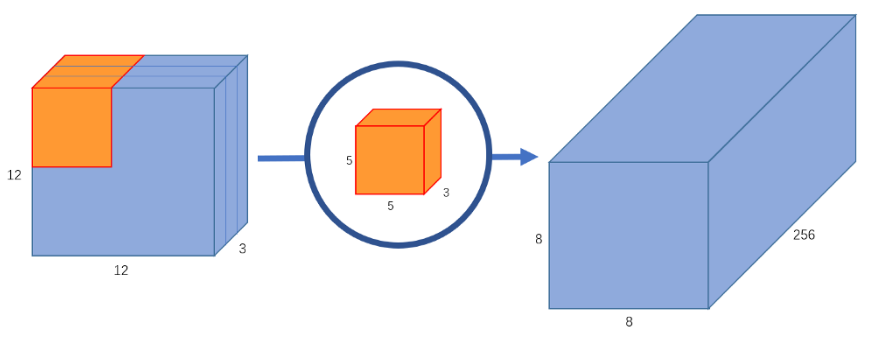
\includegraphics[width=0.8\textwidth]{img/classic_conv}
\caption{Each kernel has $k \times d$ weights. To have output of dim = $F$ we need $F$ filters $\implies F \times k \times d$ kernel weights. }
\end{figure}

\end{frame}

%--------- END Frame 12 -------------
\begin{frame}{Depthwise separable Convolutions}

\begin{figure}[h]
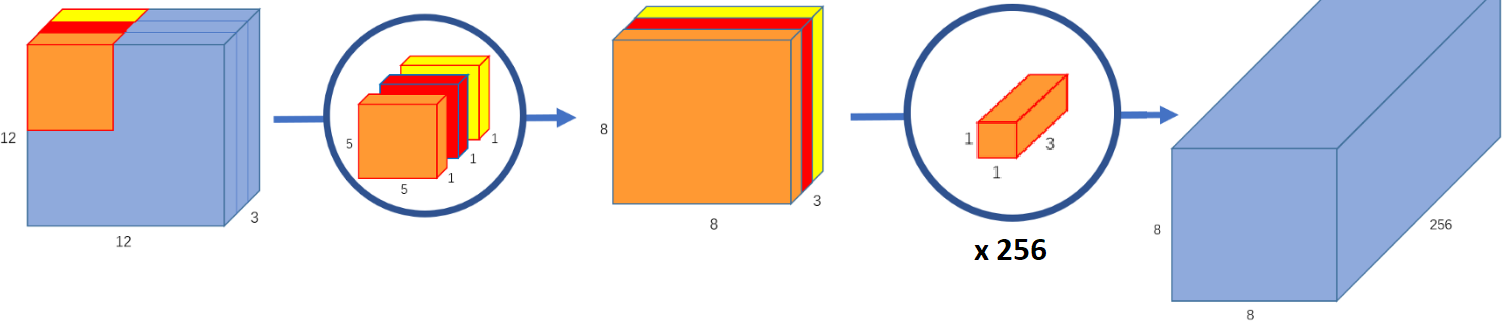
\includegraphics[width=1.0\textwidth]{img/depthwise_conv}
\caption{Use kernels of size $k \times 1$ and slide it over each channel separately = output has same number of channels as input. If we want different number of output channels (e.g. $F$) we can use $F$ efficient $1 \times 1 \times d$ filters. Resulting number of kernel weights is either just $k \times 1 \times d$ or $k \times 1 \times d + 1 \times 1 \times d \times F$ = $k \times d + F \times d$.}
\end{figure}

\end{frame}

%--------- END Frame 12 -------------
\begin{frame}{NLP case}

\begin{figure}[h]
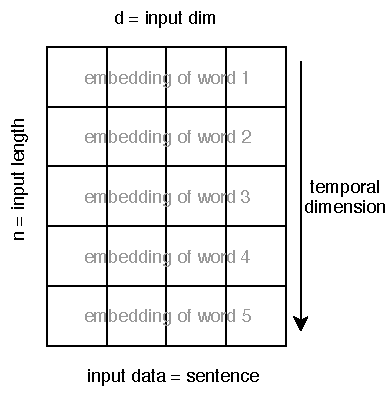
\includegraphics[width=0.5\textwidth]{img/input}
\caption{Input sentence as a matrix $X \in \mathbb{R}^{n \times d}$. }
\end{figure}
\end{frame}

%--------- END Frame 12 -------------
\begin{frame}{Depth-wise separable}

\begin{figure}[h]
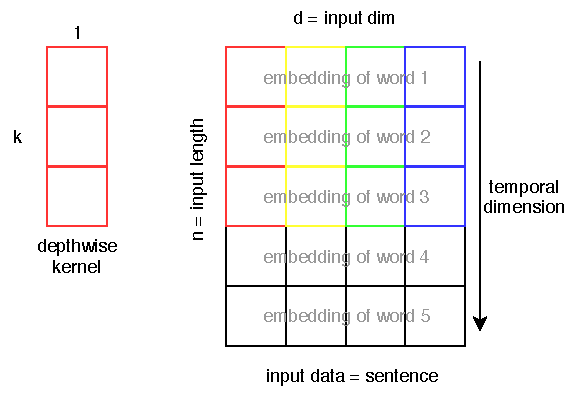
\includegraphics[width=0.6\textwidth]{img/depthwise_conv_nlp}
%\caption{Depthwise separable convolution applied to $X \in \mathbb{R}^{n \times d}$.}
\end{figure}

\begin{itemize}
\item output dim = $d$ = input dim = number of channels
\item each channel has different kernel = $d$ kernels
\item num kernel weights = $d \times k \times 1$
\end{itemize}

\end{frame}
%--------- END Frame 12 -------------
\begin{frame}{Lightweight convolutions}

\begin{figure}[h]
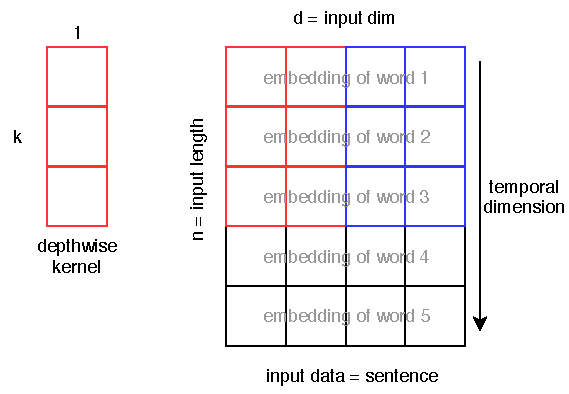
\includegraphics[width=0.6\textwidth]{img/lightweight_conv}
%\caption{Depthwise separable convolution applied to $X \in \mathbb{R}^{n \times d}$.}
\end{figure}

\begin{itemize}
\item output dim = $d$ = input dim = number of channels
\item $\frac{d}{H}$ channels share kernel weights = $H$ kernels
\item num kernel weights = $H \times k \times 1$
\item each kernel is softmaxed before being applied
\end{itemize}

\end{frame}
%--------- END Frame 12 -------------
\begin{frame}{Lightweight and dynamic convolutions}

\begin{figure}[h]
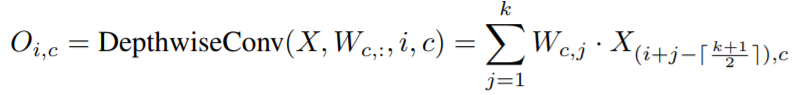
\includegraphics[width=1.0\textwidth]{img/depthwise_math}
%\caption{Depthwise separable convolution applied to $X \in \mathbb{R}^{n \times d}$.}
\end{figure}

\begin{figure}[h]
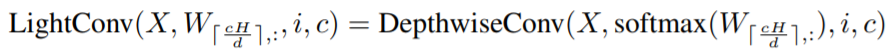
\includegraphics[width=1.0\textwidth]{img/light_math}
%\caption{Depthwise separable convolution applied to $X \in \mathbb{R}^{n \times d}$.}
\end{figure}

\begin{figure}[h]
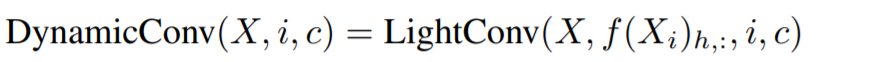
\includegraphics[width=1.0\textwidth]{img/dynamic_conv_math}
%\caption{Depthwise separable convolution applied to $X \in \mathbb{R}^{n \times d}$.}
\end{figure}

\begin{itemize}
\item dynamic = add dense layer based on $k$ elements  that generates the kernel = the kernel changes as is slides over the temporal dimension
\item dynamic weights are a function of the current time-step only rather than the entire context
\end{itemize}

\end{frame}
%--------- END Frame 12 -------------
\begin{frame}{Dynamic convolutions}

\begin{figure}[h]
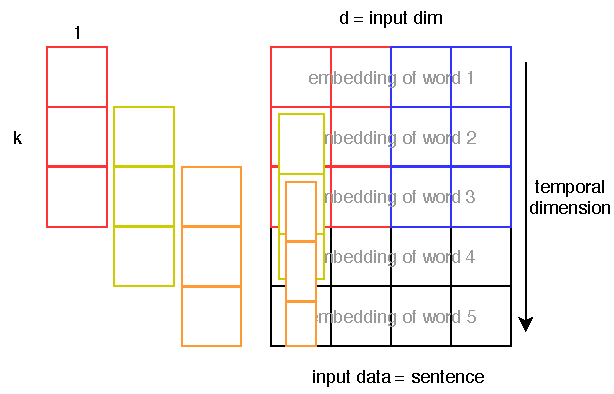
\includegraphics[width=0.6\textwidth]{img/dynamic_conv}
%\caption{Depthwise separable convolution applied to $X \in \mathbb{R}^{n \times d}$.}
\end{figure}

\begin{itemize}
\item kernel at each timestep is generated by a dense layer
\item = as kernel slides over the temporal dimension it changes
\end{itemize}

\end{frame}


%--------- END Frame 12 -------------
\begin{frame}{Comparison to attention}

\begin{figure}[h]
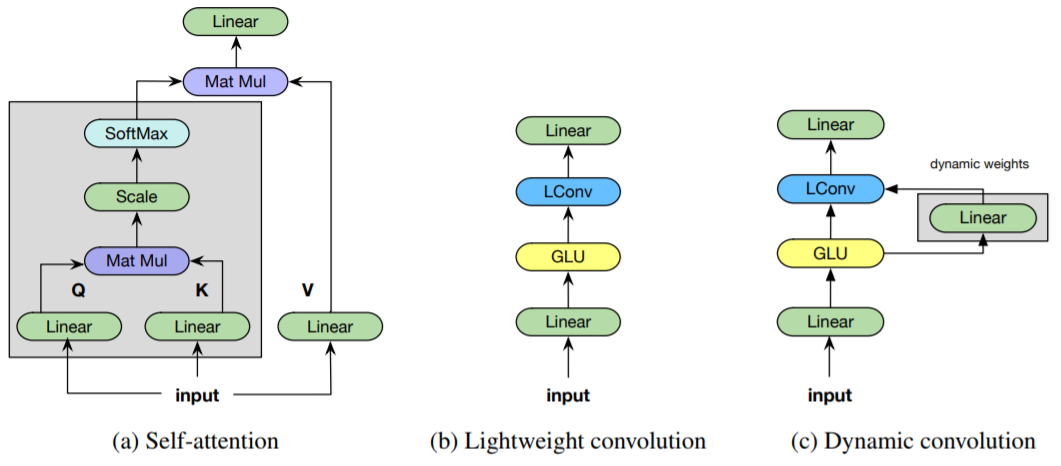
\includegraphics[width=1.0\textwidth]{img/attention}
%\caption{Depthwise separable convolution applied to $X \in \mathbb{R}^{n \times d}$.}
\end{figure}


Lightweight and dynamic  convolutions
\begin{itemize}
\item pay "attention" only to $k$ surrounding elements
\item ends with output projection to correct dim by linear layer

\end{itemize}

\end{frame}
%--------- END Frame 12 -------------
\begin{frame}{Experiments}

\begin{itemize}
\item Transformer network - replace self-attention modules with LConv or Dynamic Conv
\item LConv, DConv use less params = increase number of encoder blocks to $N = 7$ to match number of params
\item $H = 16$
\item encoder/decoder block kernels: $3, 7, 15, 31 \times 4$
\item top 3 layers of decoder have kernel size $31$
\item We train three random initializations of a each configuration and report test accuracy of the seed
which resulted in the highest validation BLEU
\item machine translation, lang. modeling, summarization
\end{itemize}

\end{frame}
%--------- END Frame 12 -------------
\begin{frame}{Results}

\begin{figure}[h]
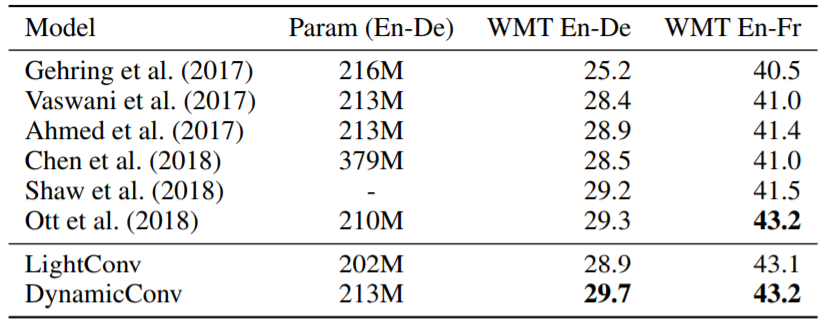
\includegraphics[width=1.0\textwidth]{img/results1}
\caption{ Machine translation accuracy in terms of BLEU for WMT En-De and WMT En-Fr on
newstest2014.}
\end{figure}
\end{frame}
%--------- END Frame 12 -------------
\begin{frame}{Results}

\begin{figure}[h]
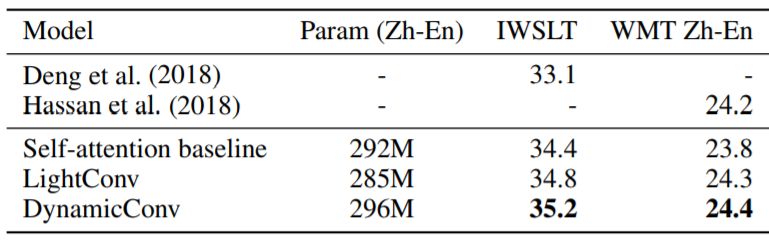
\includegraphics[width=1.0\textwidth]{img/results2}
\caption{ Machine translation accuracy in terms of BLEU on IWSLT and WMT Zh-En.}
\end{figure}
\end{frame}
%--------- END Frame 12 -------------
\begin{frame}{Results}

\begin{figure}[h]
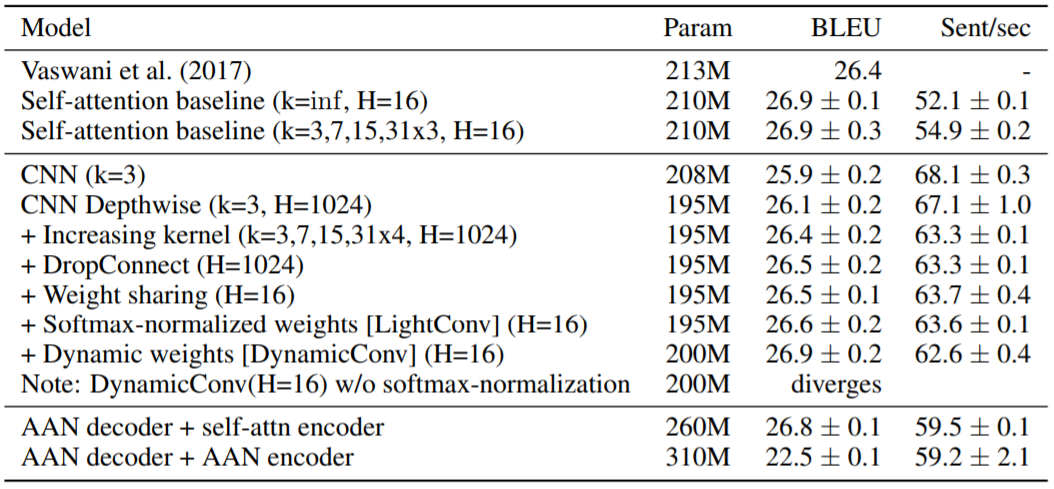
\includegraphics[width=1.0\textwidth]{img/results3}
\caption{Ablation on WMT English-German newstest2013. (+) indicates that a result includes all
preceding features. Speed results based on beam size 4, batch size 256 on an NVIDIA P100 GPU.}
\end{figure}
\end{frame}
%--------- END Frame 12 -------------
\begin{frame}{Results}

\begin{figure}[h]
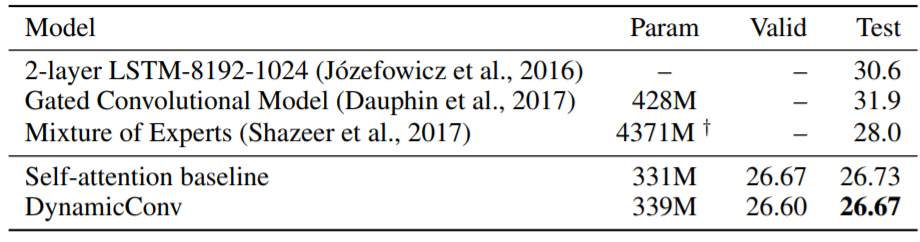
\includegraphics[width=1.0\textwidth]{img/results4}
\caption{Language modeling results on the Google Billion Word test set. + does not include embedding and softmax layers}
\end{figure}
\end{frame}
%--------- END Frame 12 -------------
\begin{frame}{Results}

\begin{figure}[h]
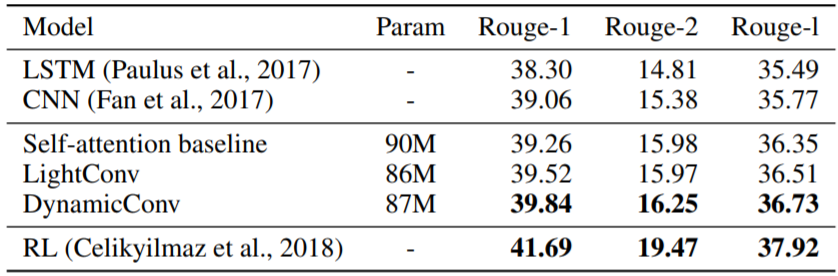
\includegraphics[width=1.0\textwidth]{img/results5}
\caption{Results on CNN-DailyMail summarization. We compare to likelihood trained approaches
except for Celikyilmaz et al. (2018).}
\end{figure}
\end{frame}

%--------- END Frame 12 -------------
\begin{frame}{Sources}

\begin{thebibliography}{0}

  \bibitem[1]{cit:lconv} 1. Wu, Felix, et al. "Pay Less Attention with Lightweight and Dynamic Convolutions." arXiv preprint arXiv:1901.10430 (2019). \url{https://arxiv.org/abs/1901.10430} 
  
  \bibitem[2]{cit:imgs} 2. Medium blogpost on depthwise convolutions. \url{https://towardsdatascience.com/a-basic-introduction-to-separable-convolutions-b99ec3102728}
  
\end{thebibliography}

\end{frame}

 
 
 
\end{document}
